% Author: PokMan Ho
% Script: res.tex
% Desc: MRes thesis result section
% Input: none
% Output: none
% Arguments: 0
% Date: Jan 2020

\documentclass[../thesis.tex]{subfiles} %% use packages & commands as this main file

\begin{document}
\section{Result}
%% text on all result -> all graphs
From Table \ref{tab:eqm}, P-only systems (eqm 3) could not give a biologically meaningful result for ``no harvest" setting under the current set of model assumptions.  Hence comparisons between with/without harvest were only done for P+B systems (eqm 4).  Comparing with/without carbon harvest in P+B systems (Fig.\ref{fig:wilcox}), the effort was statistically higher than ``no harvest" scenario only when the harvest rate was larger than 8/day.  Hence the closest significant sampled harvest rate with ``harvest" $>$ ``no harvest" was 9/day (W=57407, p=0.011).  However out of 1100 samples drew via LHS, about 90\% (n=991, median = -0.0016 (4dp)) feasible scenarios for ``no harvest" setting but only 12\% (n=134, median = 0.5670 (4dp)) for $x=9$/day.  On the other hand, P+B systems with harvest was statistically higher than their P-only counterparts for harvest rates higher than 1/day (Fig.\ref{fig:wilcox}).  At the closest significant sampled harvest rate with P+B $>$ P-only systems (2/day; W=129849, p$\ll$0.01), all (n=1100, median = -1.1334 (4dp)) scenarios were feasible for P-only system while only 25\% (n=275, median = -0.5379 (4dp)) for the P+B setting.

Effect of biological parameters on the model system (Eq.\ref{eq:ode}) was similar across different harvest rates, hence the minimal significant P+B $>$ P-only system (i.e. $x=2$/day) was selected for discussion.  P+B systems with significant beneficial log yield over ``no harvest" setting was bearing too few data for demonstration purposes due to much restricted feasible ranges on all biological parameters.  Log total carbon stored in the system for P+B was always higher than that of P-only (Fig.\ref{fig:v2}).  Within the parameter ranges, low phytoplankton growth rate (min feasible $\gP$ = 0.3472/day (4dp)) and high non-respired carbon fraction for bacterial decomposer (max feasible $\eBR$ = 0.9129 (4dp)) could crash the respective systems.  Hence no such high efficient bacteria could be considered; only a P-only scenario could be applied for low growth rate phytoplanktons.  Within feasible parameter ranges, biological parameters affect their systems differently (Fig.\ref{fig:v2}).  Generally speaking, $\ePR$, $\eP$, $\gP$ and $\mB$ had different degree of positive effect on P+B systems (and P-only systems except $\mB$); $\aP$ had a exponential decreasing effect on both P+B and P-only setting; $\eB$ and $\gB$ had a decreasing effect on P+B systems; $\eBR$ had a decreasing effect on yield but an increase in log total carbon.  Note that biological parameters for bacterial decomposer had no effect on P-only system (eqm 3 from Table \ref{tab:eqm})

\begin{figure}[H]
    \centering
    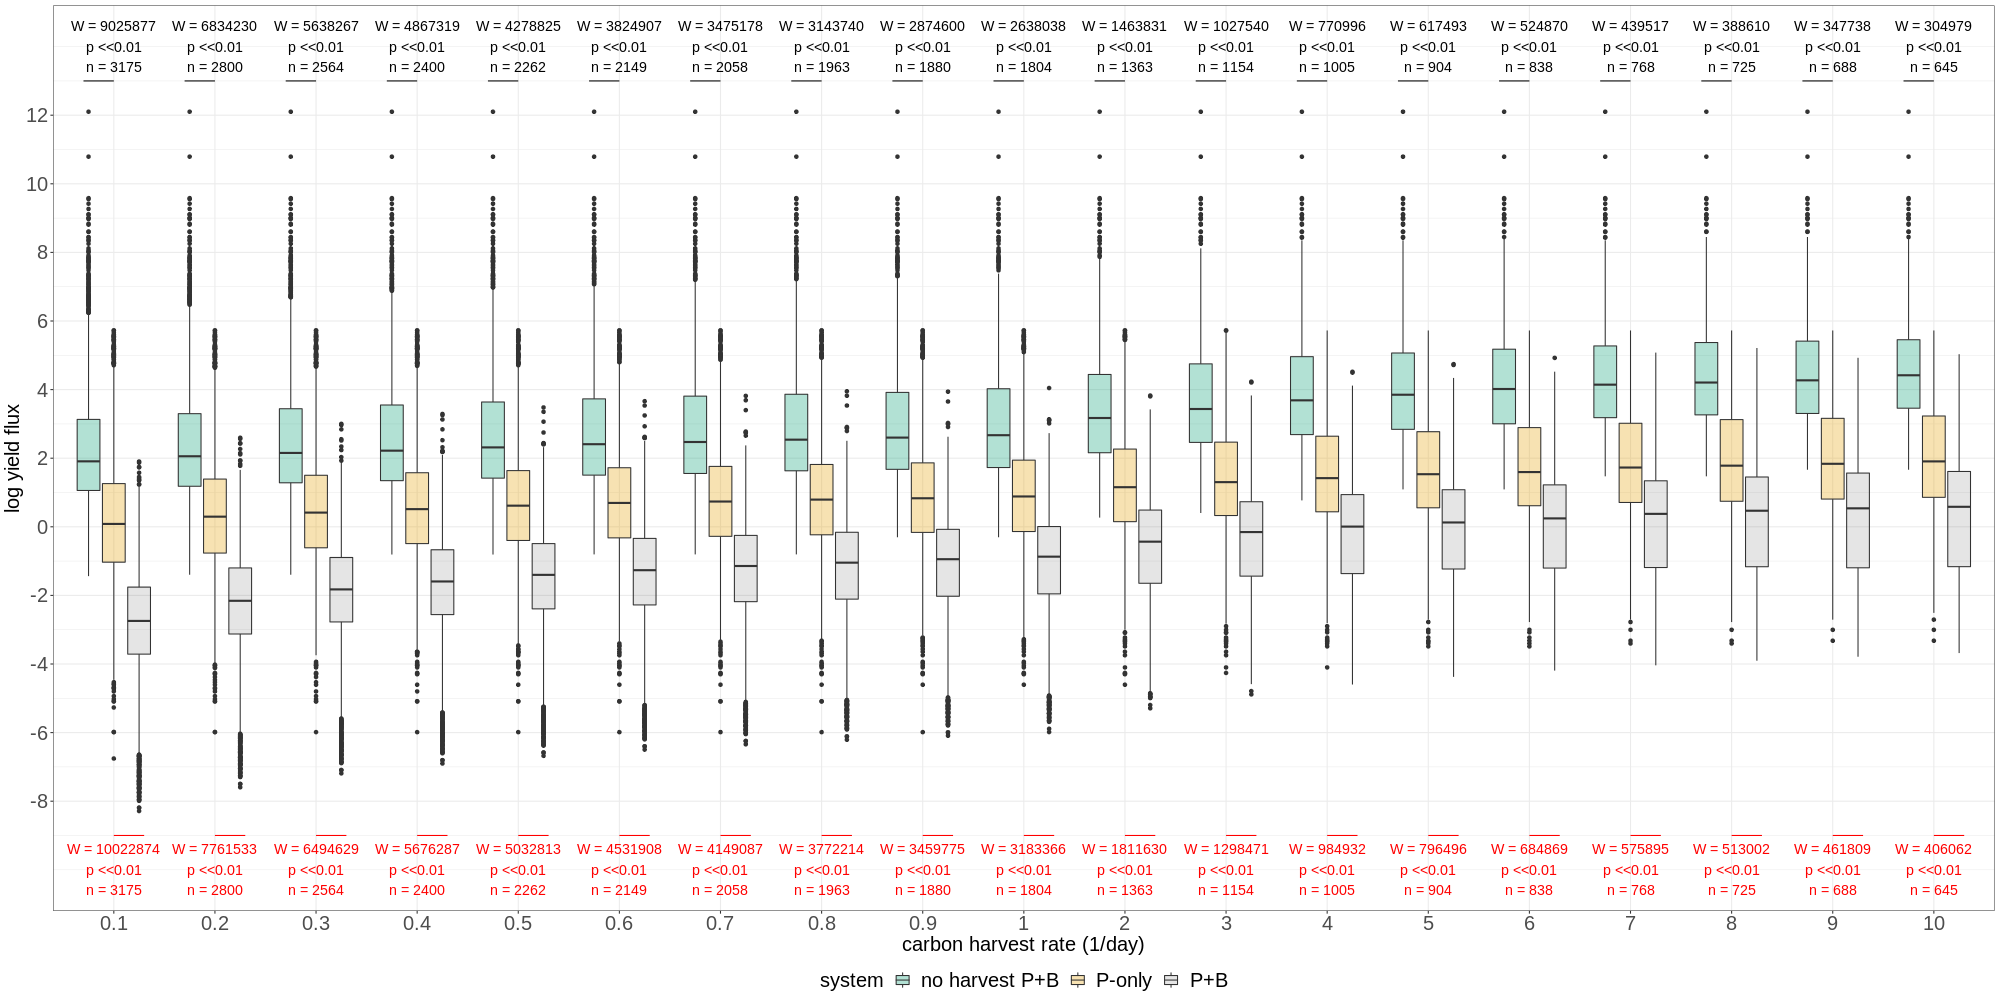
\includegraphics[width=\linewidth]{../result/Wilcox.png}
    \caption[Pairwise log yield comparisons]{Pairwise log yield distribution comparisons of P+B and P-only systems on LHS scenarios along the spectrum of harvest rates under the temperature range of 23-25\textsuperscript{o}C.  {\scriptsize Wilcox signed rank test was used on all pairwise comparisons.  Each box contained the feasible portion from identical sampled 1100 scenarios.  Sample sizes (from left to right) for P+B systems were 991 ($x=0$/day), 622 ($x=0.1$/day; vs P-only: W=474135, p$\ll$0.01; vs $x=0$: W=550431, p$\ll$0.01), 557 ($x=0.2$/day; vs P-only: W=389302, p$\ll$0.01; vs $x=0$: W=467435, p$\ll$0.01), 510 ($x=0.3$/day; vs P-only: W=335335, p$\ll$0.01; vs $x=0$: W=409589, p$\ll$0.01), 478 ($x=0.4$/day; vs P-only: W=229340, p$\ll$0.01; vs $x=0$: W=369559, p$\ll$0.01), 451 ($x=0.5$/day; vs P-only: W=271922, p$<$0.01; vs $x=0$: W=338430, p$\ll$0.01), 429 ($x=0.6$/day; vs P-only: W=250603, p=0.059 (4dp); vs $x=0$: W=312823, p$\ll$0.01), 410 ($x=0.7$/day; vs P-only: W=233841, p$>$0.1; vs $x=0$: W=292113, p$\ll$0.01), 389 ($x=0.8$/day; vs P-only: W=215958, p$>$0.1; vs $x=0$: W=270496, p$\ll$0.01), 377 ($x=0.9$/day; vs P-only: W=204167, p$>$0.1; vs $x=0$: W=256520, p$\ll$0.01), 364 ($x=1$/day; vs P-only: W=192189, p$>$0.1; vs $x=0$: W=241510, p$\ll$0.01), 275 ($x=2$/day; vs P-only: W=129849, p$\ll$0.01; vs $x=0$: W=163491, p$\ll$0.01), 233 ($x=3$/day; vs P-only: W=98399, p$\ll$0.01; vs $x=0$: W=125431, p=0.04), 209 ($x=4$/day; vs P-only: W=81793, p$\ll$0.01; vs $x=0$: W=104218, p$>$0.1), 186 ($x=5$/day; vs P-only: W=71280, p$\ll$0.01; vs $x=0$: W=91059, p$>$0.1), 163 ($x=6$/day; vs P-only: W=61205, p$\ll$0.01; vs $x=0$: W=78433, p$>$0.1), 148 ($x=7$/day; vs P-only: W=53766, p$\ll$0.01; vs $x=0$: W=69141, p$>$0.1), 143 ($x=8$/day; vs P-only: W=49749, p$\ll$0.01; vs $x=0$: W=64042, p=0.063), 134 ($x=9$/day; vs P-only: W=44383, p$\ll$0.01; vs $x=0$: W=57407, p=0.011), 126 ($x=10$/day; vs P-only: W=41090, p$\ll$0.01; vs $x=0$: W=53232, p$<$0.01) and for P-only systems were all 1100 except for harvest rate = 0/day.}}
    \label{fig:wilcox}
\end{figure}

\begin{figure}[H]
    \centering
    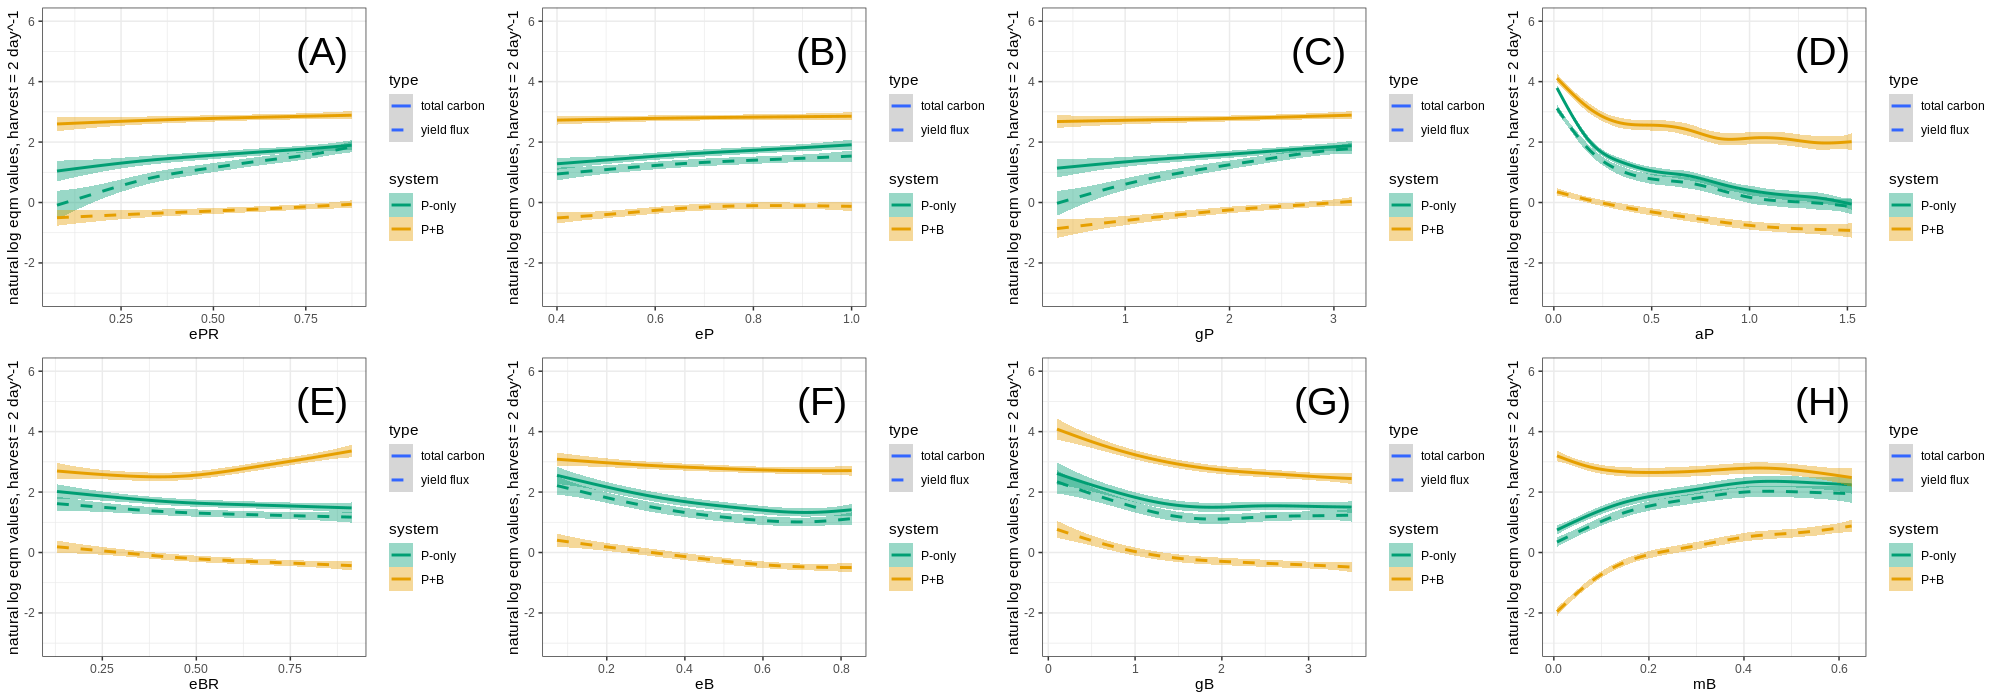
\includegraphics[width=\linewidth]{../result/var_20.png}
    \caption[Log carbon distribution for $x=2day^{-1}$ by parameter]{Distribution for ``log total carbon" (solid line) and ``log yield flux" (dash line) based on respective parameter ranges for P+B (orange) and P-only (green) systems when removal rate = 2$day^{-1}$.  {\scriptsize 95\% confidence interval for feasible LHS scenarios (N=1100) for P+B (n=275) and P-only (n=1100) systems under the temperature range of 23-25\textsuperscript{o}C.  P+B systems were significantly higher than P-only systems under Wilcox signed rank test (W=129849, p$\ll$0.01).}}
    \label{fig:v2}
\end{figure}

\end{document}
